\documentclass[a4paper]{article}
\usepackage[spanish]{babel}
\usepackage[utf8]{inputenc}
\usepackage{charter}   % tipografia
\usepackage{graphicx}
\usepackage{paralist} %itemize inline
\usepackage{underscore}
\usepackage{caratula}
\usepackage{url}
\usepackage[bottom]{footmisc}


% ********************************************************* %
% ~~~~~~~~              Code snippets             ~~~~~~~~~ %
% ********************************************************* %

\usepackage{color} % para snipets de codigo coloreados
\usepackage{fancybox}  % para el sbox de los snipets de codigo

\definecolor{litegrey}{gray}{0.94}

\newenvironment{codesnippet}{%
	\begin{Sbox}\begin{minipage}{\textwidth}\sffamily\small}%
	{\end{minipage}\end{Sbox}%
		\begin{center}%
		\vspace{-0.4cm}\colorbox{litegrey}{\TheSbox}\end{center}\vspace{0.3cm}}



% ********************************************************* %
% ~~~~~~~~         Formato de las páginas         ~~~~~~~~~ %
% ********************************************************* %

\usepackage{fancyhdr}
\pagestyle{fancy}
\renewcommand{\sectionmark}[1]{\markright{\thesection\ - #1}}

\fancyhf{}

\fancyhead[LO]{Sección \rightmark} % \thesection\ 
\fancyfoot[LO]{\small{María Carolina Gorosito, Muriel Picone Farías}}
\fancyfoot[RO]{\thepage}
\renewcommand{\headrulewidth}{0.5pt}
\renewcommand{\footrulewidth}{0.5pt}
\setlength{\hoffset}{-0.8in}
\setlength{\textwidth}{16cm}
\setlength{\headsep}{0.5cm}
\setlength{\textheight}{25cm}
\setlength{\voffset}{-0.7in}
\setlength{\headwidth}{\textwidth}
\setlength{\headheight}{13.1pt}

\renewcommand{\baselinestretch}{1.1}  % line spacing
\newcommand{\Mod}[1]{\ (\mathrm{mod}\ #1)}
% ******************************************************** %

\begin{document}

\thispagestyle{empty}
\materia{Organización del Computador II}
\submateria{Primer Cuatrimestre de 2020}
\titulo{Trabajo Práctico III}
\subtitulo{Programación de sistemas operativos: Asimilación Cronenberg}
\integrante{María Carolina Gorosito}{293/18}{kaarogor@gmail.com}
\integrante{Muriel Picone Farías}{721/18}{muri.pic@gmail.com}

\maketitle
\newpage

\thispagestyle{empty}
\vfill
\begin{abstract}
Este trabajo tiene como objetivo implementar un sistema operativo para una arquitectura Intel de 32 bits, reducido y adaptado para correr hasta 25 tareas a nivel de usuario. La implementación comprendió, a grandes, rasgos, dos aspectos diferenciados: por un lado, crear las estructuras y mecanismos generales que permiten administrar la memoria, las interrupciones y las tareas; por el otro, diseñar el funcionamiento de las tareas siguiendo la lógica de un juego inspirado en la serie Rick and Morty, considerando a las tareas como personajes en un multiverso en "memoria" que pueden controlarse unas a otras y provocar, en estas interacciones, eventos que un sistema operativo debe manejar.
\end{abstract}

\newpage
\thispagestyle{empty}
\vspace{3cm}
\tableofcontents

\newpage

\section{Introducción}

Este trabajo tiene como objetivo implementar un sistema operativo para una arquitectura Intel de 32-bits, reducido y adaptado para correr hasta 25 tareas a nivel de usuario. La implementación comprendió, a grandes, rasgos, dos aspectos diferenciados: por un lado, crear las estructuras y mecanismos generales que permiten administrar la memoria, las interrupciones y las tareas; por el otro, diseñar el funcionamiento de las tareas siguiendo la lógica de un juego inspirado en la serie Rick and Morty, considerando a las tareas como personajes en un multiverso en "memoria". \\
Cada uno jugador en el juego es representado por un par de tareas, Rick y Morty, de los universos C-137 (jugador azul) y D-248 (jugador rojo). Las tareas comenzarán posicionadas de manera aleatoria en un espacio de memoria que representa el \textit{mundo Cronenberg}. Durante el juego, estas cuatro tareas irán desplazándose con el objetivo de conquistar las mentes de la mayor cantidad de habitantes Cronenberg, ocupando espacios de memoria al mapearse a nuevas direcciones físicas y copiar allí su código. Las tareas, además, interactúan con el sistema mediante {\tt syscalls}. Estas interacciones entre las tareas y las operaciones que pueden realizar ponen en juego distintos aspectos del sistema operativo, como el intercambio de tareas, el manejo de excepciones y de otras interrupciones y el manejo de la memoria.

La implementación se realizó en diferentes etapas:
\begin{enumerate}
\item Creación de la tabla de descriptores globales (GDT), organización de la memoria con segmentación flat y pasaje a modo protegido.
\item Atención de interrupciones mediante la creación de la tabla de descriptores de interrupciones (IDT) y las rutinas de atención de interrupciones (generales, específicas del juego y también para interrupciones externas de clock y teclado).
\item Implementación de las estructuras y mecanismos necesarios para administrar la memoria utilizando paginación y crear directorios de páginas para cada tarea.
\item Definición de los segmentos de estado de las tareas (TSS) en la GDT y armado del scheduler básico.
\item Diseño de la lógica de interacción de los distintos tipos de tareas.
\item Implementación de un mecanismo de debugging para obtener detalles del contexto de ejecución al producirse excepciones en la ejecución.
\end{enumerate}

\section{Implementación}

\subsection{Infraestructura, inicio del sistema (bootloader) y modo real}

Al iniciar el equipo, se ejecuta el BIOS, que se encarga de reconocer el primer dispositivo de booteo. En este caso, el dispositivo de booteo será un floppy disk con el boot-sector. El floppy disk copia a memoria 512 bytes a partir de la dirección 0x7C00 y comienza a ejecutar el código desde allí. Luego, corren los POST, se copia el bootloader en la posición 0x1000, se copia el archivo kernel.bin a la posición 0x1200, se salta y se ejecuta el kernel. Como el boot-sector se encarga únicamente de copiar el kernel y darle el control, para cambiar el modo del procesador de modo real a modo protegido es necesario implementar una serie de estructuras que se detallan en la siguiente sección. \\
La implementación del sistema se hizo utilizando el emulador Bochs, que permite simular una computadora IBM-PC compatible desde el inicio. Además, tiene incorporado un debugger que permitió ir realizando un seguimiento de todo el proceso.

\subsection{Segmentación y pasaje a modo protegido}

\subsubsection{Tabla de descriptores globales}
Todos los sistemas deben tener una tabla de descriptores globales o GDT, que es una tabla en memoria que contiene como entradas descriptores diferentes tipos. Estos pueden ser descriptores de segmentos de memoria, descriptores de segmentos de estado de tarea (TSS), descriptores de call gate y descriptores de tablas de descriptores locales (LDT). La GDT implementada solo contiene descriptores de los primeros dos mencionados. A continuación detallaremos la estructura y funcionamiento de los descriptores de segmentos de memoria, mientras que los descriptores de TSS se describirán en la sección dedicada a la administración de tareas. \\
La GDT tiene longitud variable, y puede contener hasta $2^{13}$ o 8192 descriptores (ya que, como se verá más adelante, los selectores de segmento donde se cargan los índices de la GDT tienen 13 bits disponibles para este propósito). La tabla del sistema implementado tiene, en las primeras 8 posiciones, el descriptor nulo (de acuerdo con la convención de que el primer descriptor siempre debe serlo) y 7 entradas reservadas que no se utilizan, para cumplir con la especificación provista en el enunciado. Las siguientes 4 entradas en la tabla corresponden a dos segmentos de datos, uno de nivel 0 y otro de nivel 3, y dos segmentos de código, también de nivel 0 y 3. Estos cuatro segmentos direccionan los primeros 137 MB de memoria, y por lo tanto, implementan un modelo de \textit{segmentation flat}, que consiste en administrar la memoria como un espacio continuo, en el que los segmentos tienen el mismo tamaño y se solapan completamente en lugar de tener un tamaño variable y solapamiento parcial (como en un modelo de memoria con segmentación propiamente dicha). \\
A continuación, se encuentra definida una entrada para el segmento de video de nivel 0 para uso exclusivo del kernel, correspondiente el área de la pantalla en memoria. Este segmento se utilizará solo para las impresiones de pantalla iniciales, ya que luego toda la actividad de la pantalla se controlará desde las tareas y las estructuras que las administran. \\
Además, la GDT incluye 26 descriptores de TSS correspondientes a las tareas inicial, idle y las 24 tareas del multiverso en memoria de Rick and Morty. Estos últimos serán definidos desde funcones específicas para la administración de las tareas, por lo que no se encuentran en el archivo {\tt gdt.c}. Los 8 segmentos iniciales, los 4 de la segmentación flat, el de video y las 26 tareas dan lugar a un total de 39 entradas, por lo que se amplió el tamaño inicial de la gdt desde 35 a 50.

\begin{figure}[!htb]
  \begin{center}
	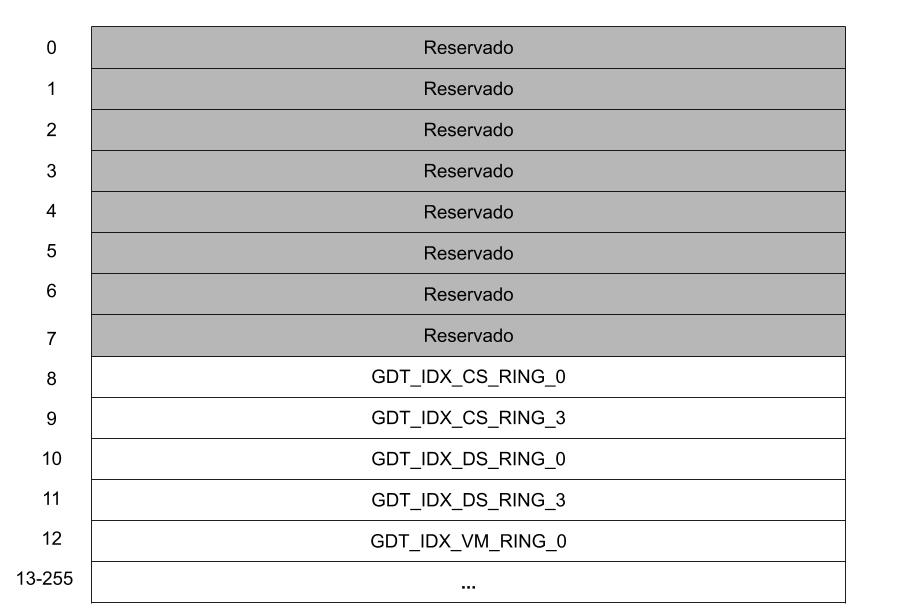
\includegraphics[scale=0.3]{img/GDT1.jpg}
	\caption{Segmentos de código y datos de la GDT}
  \end{center}
\end{figure}

\subsubsection{Estructura y contenido de los descriptores}
Cada descriptor tiene 8 bytes, organizados en la siguiente estructura que se ve en la figura 2.

\begin{figure}[!htb]
  \begin{center}
	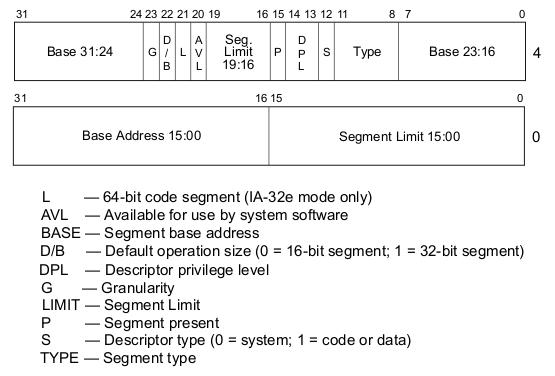
\includegraphics[scale=0.6]{img/gdtDescriptorSegmento.jpg}
	\caption{Descriptor de segmento}
  \end{center}
\end{figure}

\begin{itemize}
\item \textit{Límite y G flag (granularidad)}: campo de 20 bits especifica el tamaño del segmento. Su interpretación depende de otro campo, la G flag que indica la granularidad. Si esta se encuentra en 0, se interpreta en términos de bytes y el tamaño máximo que se puede direccionar es de 1 MB. Si está en 1, en cambio, cada incremento representa 4 KB y por lo tanto puede direccionar hasta 4 GB. Dado que el espacio de memoria a direccionar era de 137 MB, el límite de los cuatro segmentos básicos de la GDT es 0x088ff. En primer lugar, para direccionar 137 mb el bit de granularidad debe setearse en 1. 137 MB equivalen a $137\cdot2^{20}$ bytes, y como cada unidad es de 4 KB, el límite deberá ser 35072 menos uno, es decir, 0x088ff.
\item \textit{Base}: dirección de inicio del segmento, de 32 bits. En todos los casos, la posición de inicio se estableció en cero.
\item \textit{S flag}: este flag indica si el descriptor es de tipo sistema (S=0) o si se trata de un descriptor de código o datos (S=1). Dado que estos cuatro segmentos correspondían a código y datos, el valor de S es 1 para los cuatro casos.
\item \textit{Descriptor privilege level (DPL)}: especifica el nivel de privilegio del segmento y permite controlar el acceso a él, que puede ir de 0 (mayor privilegio) a 3 (menor). Como se indicó anteriormente, se definió un segmento de código y uno de datos para los niveles 0 y 3.
\item \textit{P flag}: indica si el segmento está presente.
\item \textit{Bit disponible para uso del sistema (AVL)}: en todos los casos se dejó en cero.
\item \textit{L flag}: al estar encendido, indica que un segmento de código contiene código de 64 bits. Se mantuvo en cero para todos los descriptores.
\item \textit{D/B flag}: se interpreta de diferente forma dependiendo de si se trata de un segmento de código ejecutable, un segmento de datos o un segmento de stack. Este bit siempre debe estar en 1 para segmentos de código y datos en 32 bits, por lo que se le asignó este valor a los 4 segmentos. 
\item \textit{Tipo}: campo de 4 bits que indica diferentes propiedades de un segmento según si es de código o datos, lo que se indica en el bit más significativo (0 para datos, 1 para código). En ambos casos, el bit menos significativo indica si el segmento fue accedido (se define en cero y luego el sistema lo modifica al realizar el acceso), mientras que el segundo bit menos significativo indica los permisos de lectura y escritura para los segmentos de datos y los de lectura y ejecución para los de código. El bit restante indica si un segmento de datos es \textit{expand-down} (es decir, si las direcciones de memoria deben aumentar en la dirección inversa a lo habitual, como en las pilas) o si uno de código es conforming, propiedad relacionada al sistema de protección. Dado que estas propiedades quedan fuera del alcance de esta implementación, este bit será cero en todos los casos. Se presentan los valores asociados a esta propiedad en la figura 3. En la GDT implementada los segmentos de datos tienen type {\tt 0010} y los de código {\tt 1010}, ya que ambos tendrán permisos de lectura y escritura y lectura y ejecución. 
\end{itemize}

En lo que respecta al segmento de pantalla, dado que esta tiene un tamaño de 80 x 50 píxeles, cada uno de los cuales tiene un tamaño de 2 bytes, se definió un segmento de granularidad 0 para direccionar estos 8000 bytes (con límite 0x1f3f), a partir de la dirección 0xb8000.

\begin{figure}[!htb]
  \begin{center}
	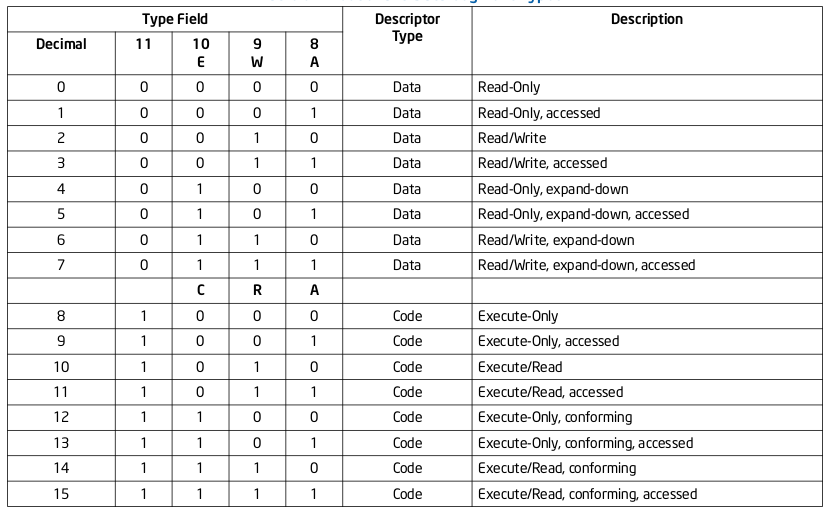
\includegraphics[scale=0.6]{img/tiposSegmentosDatosCodigo.png}
	\caption{Tipos de segmentos de datos y código}
  \end{center}
\end{figure}

\newpage

\subsubsection{Pasaje a modo protegido}
Al tener ya definida la GDT con los segmentos mencionados, se puede realizar el pasaje a modo protegido. Para esto, es necesario deshabilitar las interrupciones, activar el A20 para poder direccionar más allá del primer MB y cargar la GDT utilizando la instrucción {\tt lgdt}. Luego, se setea el bit PE del registro CR0 en 1 y se hace efectivo el pasaje a modo protegido mediante un \textit{jump far} a un segmento válido. 

\begin{codesnippet}
\begin{verbatim}

    ; Habilitar A20
    call A20_disable
    call A20_check
    call A20_enable
    call A20_check
    
    ; Cargar la GDT
    lgdt [GDT_DESC]

    ; Setear el bit PE del registro CR0
    mov eax, CR0
    or eax, 0x1
    mov cr0, eax

    jmp CS_RING_0:modo_protegido

\end{verbatim}
\end{codesnippet}

\subsubsection{Direccionamiento con segmentación}
El armado de la GDT y la definición de los segmentos es un paso previo al salto a modo protegido por el modo en que se resuelven las direcciones de memoria. Las direcciones lógicas están formadas por un selector de segmento de 16 bits y un offset de 32. Los 13 bits más significativos del selector corresponden al índice de la GDT donde se encuentra el descriptor del segmento correspondiente, mientras que los 3 bits menos significativos indican en qué tabla se encuentra (si en la GDT o en la LDT, pero a los fines de esta implementación solo utilizaremos la GDT) y el RPL o nivel de protección solicitado. Estos selectores se almacenan registros de segmento cs, ds, es, fs y gs, que al entrar en modo protegido se completan para que apunten al mismo descriptor, el del segmento de datos de nivel 0.

\subsection{Interrupt Descriptor Table}
La Interrupt Descriptor Table es una estructura que permitirá manejar las interrupciones producidas por el procesador. La misma soporta hasta 256 entradas, que serán descriptores de interrupción. Para la implementación de este sistema, se inicializó la Interrupt Descriptor Table con las entradas necesarias para poder manejar las excepciones básicas del procesador (figura 4), interrupciones externas (teclado y clock) y llamadas a sistema desde las tareas.

\begin{figure}[!htb]
  \begin{center}
	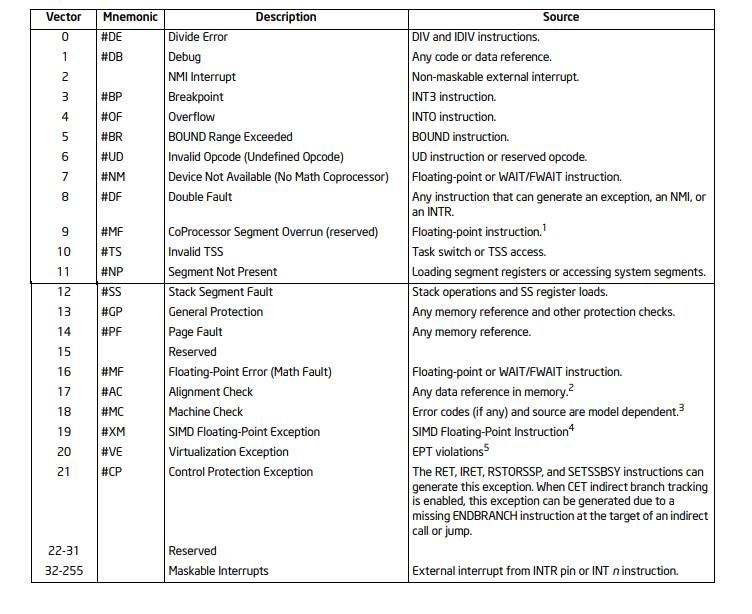
\includegraphics[scale=0.6]{img/idt.png}
	\caption{Interrupciones reservadas del procesador Intel}
  \end{center}
\end{figure}

\begin{figure}[!htb]
  \begin{center}
	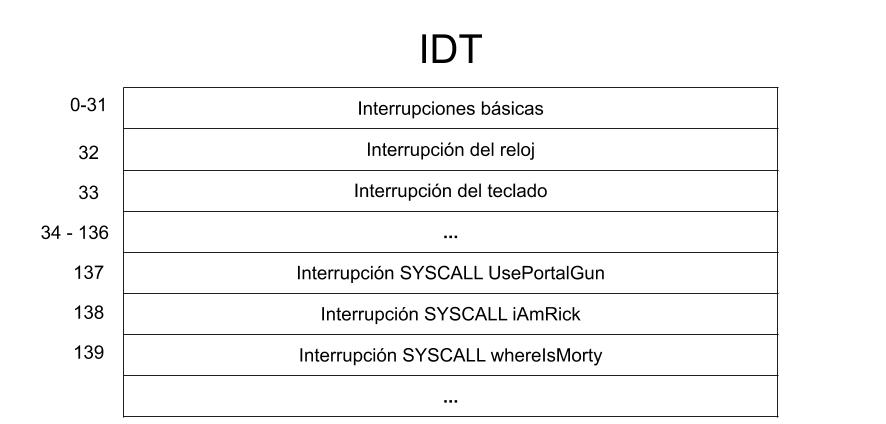
\includegraphics[scale=0.3]{img/IDTfinal.jpg}
	\caption{Estructura de la IDT implementada}
  \end{center}
\end{figure}

La implementación se realizó con las siguientes estructuras, que se encuentran en {\tt idt.h}:

\begin{codesnippet}
\begin{verbatim}

/* Struct de descriptor de IDT */
typedef struct str_idt_descriptor {
    uint16_t idt_length;
    uint32_t idt_addr;
} __attribute__((__packed__)) idt_descriptor;


/* Struct de una entrada de la IDT */
typedef struct str_idt_entry_fld {
    uint16_t offset_0_15;
    uint16_t segsel;
    uint16_t attr;
    uint16_t offset_16_31;
} __attribute__((__packed__, aligned (8))) idt_entry;

\end{verbatim}
\end{codesnippet}

En el descriptor:
\begin{itemize}
\item {\tt idt_length}: define el tamaño de la IDT en bytes-1.
\item {\tt idt_addr}: es la dirección de memoria donde comienza la IDT.
\end{itemize}

En la entrada:
\begin{itemize}
\item {\tt offset_0_15}: parte baja de la dirección del offset de la función de interrupción.
\item {\tt segsel}: selector de segmento de la función de interrupción. El DPL de este descriptor de segmento debe ser 0 para que la función {\tt iret} no produzca una excepción de tipo \textit{Page Fault} cuando se ejecute.
\item {\tt attr}: atributos de la entrada. Corresponden al bit de presente, el DPL (descriptor privilege level) que especifica el nivel de privilegio mínimo que debe tener el llamado a la interrupción y el bit S (Storage Segment) que debe estar seteado en 0 para las interrupciones.
\item {\tt offset_16_31}: parte alta de la dirección del offset de la función de interrupción.
\end{itemize}

Una vez inicializada la IDT, es necesario cargarla desde el kernel con la instrucción {\tt lidt}. En un inicio, las interrupciones se manejaban mostrando por pantalla el código del problema que se produjo y luego se interrumpía la ejecución, pero posteriormente se modificaron estas rutinas para que en caso de producirse una excepción en una tarea de nivel 3, se resuelva el problema y se desaloje a la tarea que lo produjo. En caso de producirse un error en el kernel, se mostrará el código de error. \\
Las interrupciones 32 y 33 corresponderán a interrupciones externas (clock y teclado, respectivamente), cada una estará declarada en la IDT y tendrá su rutina de atención. Para que el kernel pueda atenderlas, se debe remapear el PIC y activar las interrupciones con el comando {\tt sti}. Cuando la interrupción sea del teclado, obtendremos además un \textit{scan code} que nos indica cuál es la tecla que está siendo pulsada, lo que utilizaremos para imprimir en esquina superior derecha de la pantalla cualquier número del 0 al 9 que se presione. Posteriormente, servirá también para habilitar el modo debug al apretar la tecla "Y". \\
En principio, las rutinas de atención detenían la ejecución y se quedaban en un ciclo infinito, imprimiendo por pantalla el código de excepción producido, sin embargo más adelante en nuestra implementación se modificó de modo que se desalojen las tareas que causan excepciones y se pueda retomar la ejecución.

\subsection{Paginación}

\subsubsection{Directorio y tablas de páginas}
Para completar la administración de la memoria, se implementaron las estructuras necesarias para poder activar paginación. En líneas muy generales, la paginación consiste en dividir la memoria en fragmentos de 4 KB y acceder a ellos mediante una tabla en la que se almacena la información de cada uno de ellos (la dirección física donde comienza el fragmento y sus atributos). Cada una de estas entradas tiene 4 bytes y cada tabla ocupa 4 KB en memoria, por lo que cada una puede tener hasta 1024 entradas. A su vez, las direcciones donde se encuentran estas tablas se almacenan en un directorio de tablas de página, que no es más que otra tabla pero en lugar de almacenar en sus entradas las direcciones físicas donde comienzan los fragmentos de memoria, almacena las direcciones donde se encuentran las tablas. De esta manera, se pueden definir 1024 tablas, que permiten direccionar 4 GB de memoria. \\
Las direcciones lineales de memoria están formadas sobre la base de estas estructuras: los 12 bits menos significativos corresponden al offset dentro de la página en memoria, los 10 siguientes al índice de la entrada en la tabla correspondiente y los 10 más significativos al índice de la entrada de la tabla en el directorio. Así, segmentando de esta forma una dirección lineal, es posible hacer todo el recorrido y recuperar su dirección física. \\
Para poder activar paginación, se mapearon con \textit{identity mapping} los primeros 4 MB, correspondientes al kernel y al área libre de kernel, de acuerdo con lo requerido por el enunciado. Realizar el mapeo de esta manera significa que la dirección lineal y la física coinciden, ya que es posible elegir las entradas en el directorio y en la tabla para que esto ocurra. En este caso, dado que el rango a mapear es 0x00000000-0x003FFFFF usando \textit{identity mapping} y corresponde a los primeros 4 MB de memoria, la tabla utilizada fue la entrada 0 en el directorio y se mapearon todas sus páginas. \\

\begin{figure}[!htb]
  \begin{center}
	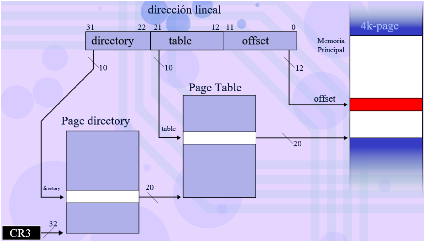
\includegraphics[scale=0.6]{img/esquemaPaginacion.png}
	\caption{Esquema de traducción de dirección lineal a dirección física}
  \end{center}
\end{figure}

\subsubsection{Memory Management Unit}
El sistema cuenta con una Memory Management Unit (MMU), implementada en mmu.c. Este mapeo inicial se realizó mediante la función {\tt initKernelDir}. Como se indica en el enunciado, el directorio de páginas del kernel fue ubicado en la dirección 0x27000 y las tabla de páginas se encuentran a partir de la dirección 0x28000.
La MMU, además de inicializar el directorio de páginas del kernel, será la encargada de inicializar los directorios de páginas para las tareas, ya que cada una tendrá un mapa de memoria propio. Esto se realiza en la función {\tt initTaskDir}. \\
initTaskDir recibe como parámetros una dirección física del mundo Cronenberg, es decir, del área donde se moverán las tareas, la dirección donde se encuentra el código fuente de la tarea y los atributos cono los que deberán mapearse las páginas. Cada tarea ocupa 8 KB (allí estarán tanto su código como la pila correspondiente). Por este motivo, es necesario mapear dos páginas. Todas las tareas se mapean a la dirección virtual 0x8000000. Además, también deberá estar mapeado el kernel, ya que se deberá atender las interrupciones. Para evitar realizar otro mapa de memoria para el kernel, se implementó una optimización ubicando en el nuevo directorio la tabla del kernel definida originalmente. Luego de mapear las páginas, esta función también realiza la copia del código desde la fuente a la posición mapeada. Para ello, mapea la dirección física al CR3 del kernel usando \textit{identity mapping} para poder copiar el código y luego la desmapea. Finalmente, devuelve la dirección del directorio de páginas para cargar en el cr3. \
Para poder realizar las operaciones descritas arriba, la MMU cuenta con una variable global que almacena la próxima página libre del kernel y permite obtenerla mediante la función nextFreeKernelPage, y de esta manera es posible ir obteniendo nuevas posiciones de memoria donde guardar las nuevas páginas necesarias para crear nuevos directorios y tablas. Además, también incluye las funciones mapPage y unmapPage, que permiten mapear y desmapear páginas como se mencionó anteriormente. \\
En cuanto a los atributos de las páginas, vale la pena señalar que en los directorios se optó por los permisos menos restrictivos, ya que estos tienen precedencia. De esta manera, se puede restringir ls permisos desde las entradas de las páginas de manera independiente, sin correr el riesgo de que haya un override de permisos impuestos desde el directorio. \\
Una vez armado el directorio para el kernel, desde {\tt kernel.asm} se carga su dirección en el CR3 y se enciende el bit correspondiente en el registro CR0 para activar paginación. La creación de directorios para las tareas se realiza desde las estructuras específicas para la administración de tareas, que se verán más adelante.

\subsection{Administración de tareas}
Una tarea es un proceso que ejecuta una instancia de un programa. Como se indicó más arriba, para que las tareas puedan funcionar en un sistema es necesario contar con ciertas estructuras y mecanismos. Una tarea debe poder ser ejecutada, desalojada e intercambiada por otra. La arquitectura provee algunos mecanismos para realizar estas operaciones, pero hay otros que deben ser implementados. \\
El sistema implementado comienza ejecutando una tarea, llamada \textit{idle}, que no realiza ninguna operación sobre la memoria. Esta tarea funciona como una tarea default a la que se puede acudir para poner el sistema en modo espera, por ejemplo, cuando se produce una excepción. Luego, utiliza un esquema \textit{round-robin} para intercambiar tareas, ejecutando una tarea diferente en cada ciclo de clock, siguiendo un orden preestablecido.

\subsubsection{Task State Segment}
Al intercambiar tareas, es necesario almacenar información sobre su contexto para poder volver a ella en su próximo turno y retomar la ejecución sin perder información y sin que se produzcan fallas. Esto se logra guardando toda la información relacionada con el contexto de ejecución en un espacio en la memoria. Como se mencionó al describir la GDT, la arquitectura provee un tipo de descriptor de segmento específico para estos segmentos de memoria, los segmentos de estado de tarea. Estos segmentos tienen un tamaño mínimo de 104 bytes y una estructura fija, que puede verse en la figura 6.

\begin{figure}[!htb]
  \begin{center}
	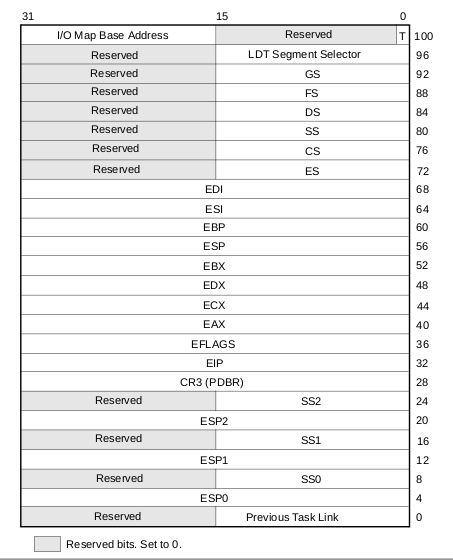
\includegraphics[scale=0.6]{img/tssEstructura.png}
	\caption{Estructura de los segmentos de estado de tarea (TSS)}
  \end{center}
\end{figure}

En la implementación la creación de los TSS y la definición de las entradas correspondientes en la GDT se realiza desde {\tt tss.c}. La funcion {\tt tss_init} crea ambas estructuras para todas las tareas del mundo Cronenberg a partir de su {\tt id} y su {\tt cr3}. Esta función completa el TSS ubicando el eip en la dirección de inicio del código y la pila al final de los 8 KB asignados a cada tarea, habilitando las interrupciones en {\tt eflags}, completando los selectores de segmento con los offsets en la GDT correspondientes a los segmentos de código y datos definidos, deshabilitando las interrupciones de I/O map y asignando una página nueva del área libre de kernel para la pila de nivel 0 (en caso de que se produzcan interrupciones y haya cambios de privilegio). En la GDT, crea una entrada de 104 bytes a partir de una dirección definida por el compilador. \\
Además, en {\tt tss.c} también se encuentran las funciones {\tt tss_init_idle} y {\tt tss_init_initial}, que inicializan las dos tareas restantes. La tarea inicial se encuentra vacía ya que se utiliza una única vez al iniciar el scheduler desde el kernel, haciendo un {\tt jmp far} de la tarea inicial a la idle. \\
Por otro lado, {\tt tss_init} lo usaremos para inicializar las tareas de Rick C137, Rick D248, Morty C137, Morty D248 y todos los Cronenbergs (sin conquistar), esta función toma un CR3 para setearlo como CR3 de la TSS y genera una entrada en la GDT según el id de la tarea a la que le estemos creando el descriptor de segmento.

\subsubsection{Scheduler}
Para que funcione el juego, necesitamos una una estructura dentro del sistema operativo que se encargue de intercambiar las 24 tareas necesarias y que cada jugador pueda moverse. Esta estructura será el scheduler, que se encargará de inicializar las 24 tareas, decidir la siguiente tarea a ejecutar y de guardar la información del procesador durante la ejecución de cada tarea para el modo debug. \\
Para implementar el scheduler se crearon una lista de {\tt struct task} con información sobre las tareas y la función {\tt sched_init}, donde se inicializa la información de {\tt taskInfo} para cada tarea. Esta información será utilizada tanto en el juego, para almacenar las posiciones de cada tarea en el tablero, como para la administración de las tareas a nivel sistema, ya que tiene el CR3 correspondiente y su índice en la GDT. Además, también incluyen su status, que permitirá que el scheduler las saltee si ya no están activas.

\begin{codesnippet}
\begin{verbatim}

typedef struct taskInfo {
    e_taskType_t type;
    uint8_t status;
    uint8_t x;
    uint8_t y;
    uint8_t gdt_index;
    uint32_t cr3;
} __attribute__((__packed__, aligned (8))) task;

\end{verbatim}
\end{codesnippet}

La función {\tt sched_init}, además, inicializa el TSS de cada tarea usando la función {\tt tss_init} explicada anteriormente. Para ponerlo en ejecución, basta con llamar esta función desde el kernel y ya comenzará su trabajo de saltar de tarea en tarea: cada vez que se atienda una interrupción del clock del sistema, en caso de que no haya terminado el juego, se llamará a {\tt sched_nextTask}, que se va a encargar de devolver el índice de la GDT de la siguiente tarea para poder obtener el selector de segmento y saltar a ella mediante un {\tt jmp far}. \\
Esta función {\tt sched_nextTask} es crucial para el correcto funcionamiento del scheduler, la misma se encarga de saltar de tarea tomando el valor de la variable global {\tt currentTaskId}, que indica qué tarea está ejecutándose actualmente por su posición en la {\tt taskList}, y actualizándolo por el siguiente índice de una tarea que \textit{no} esté muerta. En caso de estarlo, simplemente se la saltea y ejecuta la próxima viva.

\subsection{Juego}
Como se mencionó en la introducción, el funcionamiento de las tareas en este sistema operativo está inspirado en la serie Rick and Morty. La ejecución de tareas simula un juego entre dos jugadores, cada uno representado por un par de tareas, Rick y Morty, de los universos C-137 (jugador azul) y D-248 (jugador rojo). Las tareas comenzarán posicionadas de manera aleatoria en un espacio de memoria que representa el mundo Cronenberg. El objetivo será conquistar las mentes de la mayor cantidad de habitantes Cronenberg, algo que las tareas podrán lograr desplazándose para mapearse a nuevas direcciones físicas y copiar allí su código. Así, tendrán la posibilidad de modificar el espacio de otra tarea y conquistarla. Si en alguna de estos movimientos alguna de las tareas falla, el personaje asociado morirá, y no podrá ser revivido.
El juego termina si se cumple alguna de las siguientes condiciones:
\begin{itemize}
\item Alguno de los Ricks captura todas las mentes y el otro no tiene ninguna
\item Alguno de los Ricks o Mortys muere o es capturado por alguien del equipo contrario
\item Mueren todos los Cronenbergs (en este caso el juego no tiene ganador)
\end{itemize}

\subsubsection{Estado inicial del juego}
Los 24 personajes se ubicarán en distintas posiciones del mundo Cronenberg, definidas en un arreglo con valores para las coordenadas x e y en {\tt task.h}. Cada personaje/tarea tiene un id único que lo identifica en la lista de tareas creada en el scheduler, y este id se utilizará para identificarlos a lo largo de todo el juego. \\
Este arreglo de tareas contiene información sobre el tipo de tarea, que en estado inicial es el correspondiente a cada personaje (aunque irá cambiando a lo largo del juego). Todos los Cronenbergs comienzan libres. Además, todos los personajes comienzan libres, ya que una vez muertos no pueden ser revividos. \\
Ambos jugadores comienzan con sus puntajes en cero, que son almacenados en una variable global en {\tt game.c}. También se cuenta con un contador de Cronenbergs vivos, que se utiliza para controlar si terminó el juego y quién es el ganador.

\subsubsection{Desarrollo del juego (syscalls)}
Para conquistar mentes, los Ricks y los Mortys cuentan con herramientas que toman la forma de llamados al sistema. Estas herramientas son tres y se describen a continuación.
\\
\\
\textbf{usePortalGun}:
La única manera que tienen los personajes de moverse por el mundo es utilizar un arma de portales. La syscall {\tt usePortalGun (int 137)} toma como parámetros una posición relativa representada por {\tt x} e {\tt y}, un parámetro {\tt cross} (que indica el tipo de desplazamiento que realizará el personaje) y un parámetro {\tt withMorty} (que indica si se desplazará uno o los dos). \\
El uso de esta herramienta tiene las siguientes restricciones:
\begin{itemize}
\item Solo pueden usarla Rick o Morty. Si un Cronenberg intenta usarla, no tendrá ningún efecto (es decir, el Croneberg no podrá desplazarse pero tampoco le hará daño intentarlo).
\item Rick solo puede usar el arma una vez por turno. La primera vez que la usa se activa un flag que indica que ya la utilizó, y al iniciarse un nuevo turno este flag se limpia.
\item Morty solo podrá utilizar el arma por cada 10 usos que haya hecho el Rick de su equipo. En la implementación, se dispone de un contador de los usos que realizó Rick del arma hasta el momento. Si estos son más de 10, Morty podrá usar el arma pero cada vez que la use se restarán 10 a este contador. Esto permite que Morty no pierda oportunidades de usar el arma si en un turno no logró utilizarla por algún motivo, ya que son acumulables.
\end{itemize}

El parámetro {\tt withMorty} puede tomar los valores 1 o 0. Si es 1 y el que está utilizando el arma es Rick, Morty se desplazará con él, es decir, se moverá la misma cantidad de posiciones en los ejes x e y. En caso contrario, se quedará en su lugar. Si este parámetro tiene valor 1 pero es Morty quien está usando el arma, no tendrá efecto, ya que solo se moverá Morty. Para desplazar a Morty desde el mapa de memoria de Rick, se optó por cargar el cr3 de la tarea Morty momentáneamente para hacer el mapeo correspondiente y luego volver a cargar el cr3 de Rick. \\
El parámetro {\tt cross} indica si el personaje creará un portal en la posición indicada ({\tt cross=0}) o si se desplazará efectivamente. En términos de las operaciones en memoria, crear un portal significa  mapear la dirección física destino del portal a partir de la 0x08002000. Esto permite al personaje que usó el arma poder acceder a ese espacio de memoria para leerlo o escribirlo, y así ponerle código que mate o conquiste a otro personaje ubicado allí. Un punto importante a señalar es que cada personaje podrá tener un portal creado a la vez, es decir que si crea un nuevo portal, este también se mapeará a 0x08002000, borrando el anterior. \\
Para llevar un registro de los portales creados por cada personaje, se cuenta con un arreglo de {\tt structs portalInfo} que contienen las posiciones x e y. Cada vez que un personaje crea un nuevo portal, la información se actualiza allí. Las posiciones corresponden a los id de los personajes, al igual en la lista de tareas (por ejemplo, RickC137 y su portal ocuparán la primera posición y su id será 0 en ambas listas). \\
Si cross es 1, se copia el código del personaje a la dirección destino y luego se mapea allí (y se desmapea de la anterior) para seguir ejecutando desde allí. Cuando esto ocurre, se actualiza la posición del personaje en la lista de tareas.
\\
\\
\textbf{whereIsMorty}:
La syscall {\tt whereIsMorty} puede ser utilizada para obtener la posición de Morty en relación con la de Rick, es decir, la distancia entre ellos. Para poder identificar la dirección del desplazamiento, no se tomaron los valores absolutos de esta distancia sino que se optó por preservar el signo. Todos los personajes pueden llamar a esta syscall, pero solo tendrá efecto si es usada por Rick. \\
En cuanto a la implementación, retorna en el registro {\tt eax} la cantidad de celdas en "x" y en {\tt ebx} la cantidad de celdas en "y". Para esto, en el código de atención de interrupción en {\tt isr.asm} se crean dos punteros a partir de etiquetas en asm y se pasan como parámetro a una función en {\tt game.c} que devolverá los valores calculados.
\begin{codesnippet}
\begin{verbatim}
    pushad 
    push morty_coord_y    ; tag donde se guardará el valor de x
    push morty_coord_x    ; tag donde se guardará el valor de y
    call game_whereIsMorty
    add esp, 8
    popad
    mov eax, [morty_coord_x]
    mov ebx, [morty_coord_y]
    iret
\end{verbatim}
\end{codesnippet}

\textbf{iAmRick}:
Esta syscall puede ser utilizada por todos los personajes para informar a qué universo/equipo pertencen (el código del universo es pasado por parámetro). Naturalmente, los Rick y Morty del universo C-137 la llamarán con su propio código y lo mismo harán los del universo D-248, a menos que sufran modificaciones en su código. Cuando un personaje informa al sistema su pertenencia, si es diferente a la actual se modificara su tipo de tarea en la lista, y esto afectará el desarrollo del juego. Si un Cronenberg utiliza iAmRick, se considerará conquistado; de hecho, forzarlo a usar esta syscall con el código del jugador es la única forma de lograr conquistarlo. El juego continuará y el jugador que realizó la conquista sumará un punto. Si un Rick o un Morty llaman a esta syscall con el código contrario al que le corresponden, también se considerarán conquistados pero en este caso el juego terminará y ganara el jugador contrario. \\
Vale la pena señalar que se decidió que los Cronenbergs no puedan ser reconquistados, por lo que una vez que son una tarea de tipo Cronenberg D-248 o Cronenberg C-137, no pueden cambiar. Por este motivo, la función que implementa esta syscall solamente chequea si la tarea que llamó al servicio es de tipo Cronenberg (sin conquistar) para asignarle el tipo de tarea que corresponde.

\subsection{Pantalla}
Como se mencionó anteriormente, la pantalla tiene un tamaño de 80 x 50 píxeles, cada uno de los cuales tiene un tamaño de 2 bytes. Al describir la implementación de la GDT, se indicó que se definió una entrada para un descriptor de segmento de video para pintar en la pantalla, que fue utilizado únicamente para imprimir por pantalla el tablero del juego, y a partir de ese punto se utilizaron funciones en C para imprimir por pantalla las estructuras relacionadas a las tareas y la lógica del juego, por lo que terminaremos utilizando el segmento de datos nivel 0 y el anterior queda en desuso. \\
Para entender como funcionan las funciones de impresión de pantalla, hay que tener en cuenta que cada pixel tiene un byte que corresponde a un "back colour", que corresponde al color del fondo, y un "fore colour", que es el color que corresponderá al caracter a imprimir. Por esto, en la clase {\tt colors.h} definimos los colores alternando el nibble del back colour y el nibble del fore colour hasta obtener los dos bytes que corresponden al pixel. En principio, imprimimos los números de libreta por pantalla usando la función {\tt screen_printNumeroLibreta}, que a su vez usa la función {\tt print} usando como parámetros nuestros números de libreta, coordenadas x e y correspondientes a la esquina superior izquierda de la pantalla, y como atributo el color "WHITE_ON_PINK" (0xDFDF) que imprime letras blancas con fondo rosa, que es el color de nuestro tablero de juego. \\
Luego, se implementaron funciones para imprimir por pantalla todo lo necesario para inicializar el juego. En la función {\tt game_init} del archivo {\tt game.c}, primero se limpia el tablero para que esté todo de color uniforme. Después, se imprimen los puntajes de los jugadores rojo y azul con la función {\tt screen_printPlayerScores}, que en este caso será 0 porque está recién comenzando el juego, y se imprime en el pie del tablero el estado inicial de todos los Cronenbergs con la función {\tt screen_printCronenbergTable}. En principio, estarán todos vivos y sin conquistar, por lo que todos tendrán el status "C", pero a medida que avance el juego, podrán cambiar a "B" si fueron conquistados por el jugador azul, "R" si su mente fue conquistada por el jugador rojo o "X" si están muertos. Por otro lado, la función {\tt screen_drawTasks} dibuja las tareas en el tablero según sus coordenadas x e y, información que guardan en su estructura previamente calculada en el archivo {\tt sched.c}, según el tipo de tarea que sea (si corresponde a alguna tarea del mundo C-137 se imprimirán de color rojo, si pertencen al mundo D-248 serán de color azul y si pertenecen al mundo Cronenberg serán de color verde, además de imprimirse con la letra "R" si se trata de una tarea de tipo Rick, "M" si se trata de un Morty y "C" si se trat de un Cronenberg). Además, esta función dibuja también los portales activos, marcándolos en el mapa los portales con un "@" de color celeste. Cabe resaltar que cada tarea ocupa un píxel: como el tamaño de la pantalla es de 80x40, el total de celdas del tablero es 3200 bytes; como cada dirección física está entre 0x400000 y 0x1CFFFFF, $0x1D00000 - 0x400000 / 0x2000 = 3200$ (0x2000 corresponde a 8 kb, tamaño de las tareas). \\
Cada vez que ocurre una interrupción de reloj, se llamará a la función {\tt game_updateScore}, que, en caso de haberse desplazado alguna tarea en el tablero, se encargará de limpiarlo e imprimir el nuevo status de los Cronenbergs con la función ya mencionada y volver a dibujar las tareas en el tablero. También, chequeamos si terminó el juego. En caso de ser así, se imprime por pantalla un recuadro gris que indica cuál es el jugador que ganó (o si murieron todos los Cronenberg) con la función {\tt screen_printEndOfGame}.
\begin{figure}[!htb]
  \begin{center}
	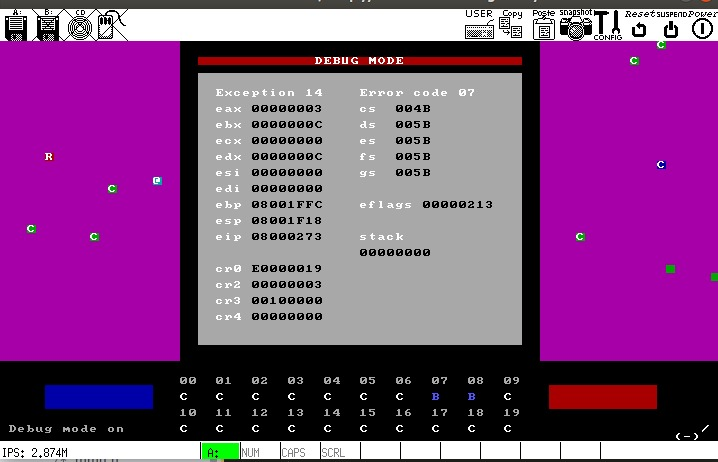
\includegraphics[scale=0.4]{img/modoDebug.png}
	\caption{Ejemplo de pantalla de error}
  \end{center}
\end{figure}

En lo que respecta al modo debug, al tenerlo activado y producir una excepción, se imprime por pantalla un recuadro que indica la excepción del procesador que ocurrió. Esto se hace con la función {\tt screen_printDebugBox}, que toma la información guardada en la estructura {\tt debugInfo} para mostrar el estado del procesador.


\section{Modo debug}
Como ya se indicó, al presionar {\tt Y} el sistema activa el modo debug, que al producirse una excepción muestra en pantalla un detalle de todo el estado del procesador en ese momento. El juego detiene su ejecución y se mantiene esta pantalla hasta presionar nuevamente la tecla {\tt y}, que hace desaparecer la pantalla y reanuda el juego. El modo debug quedará desactivado hasta que se vuelva a presionar {\tt y}. Se indica si el modo debug está activado en el extremo inferior izquierdo de la pantalla.

\end{document}